\begin{frame}
    \frametitle{前情回顾}
    \begin{itemize}
        \item 光场量子化~~真空态~~数态~~产生湮灭算符 
        \item 相干态~~压缩态~~辐射场 
        \item 光子计数 ~~ 关联函数~~反聚束
        \item 光场表象
        \item 光与原子相互作用
    \end{itemize}     
\end{frame}

%%%%%%%%%%%%%%%%%%%%%%%%%%%%%%%%%%
\begin{frame} [plain]
    \frametitle{}
    \Background[1] 
    \begin{center}
    {\huge 第17-18讲:光腔中的原子}
    \end{center}  
    \addtocounter{framenumber}{-1}   
\end{frame}


\begin{frame} 
\frametitle{引入}
  \begin{center}
       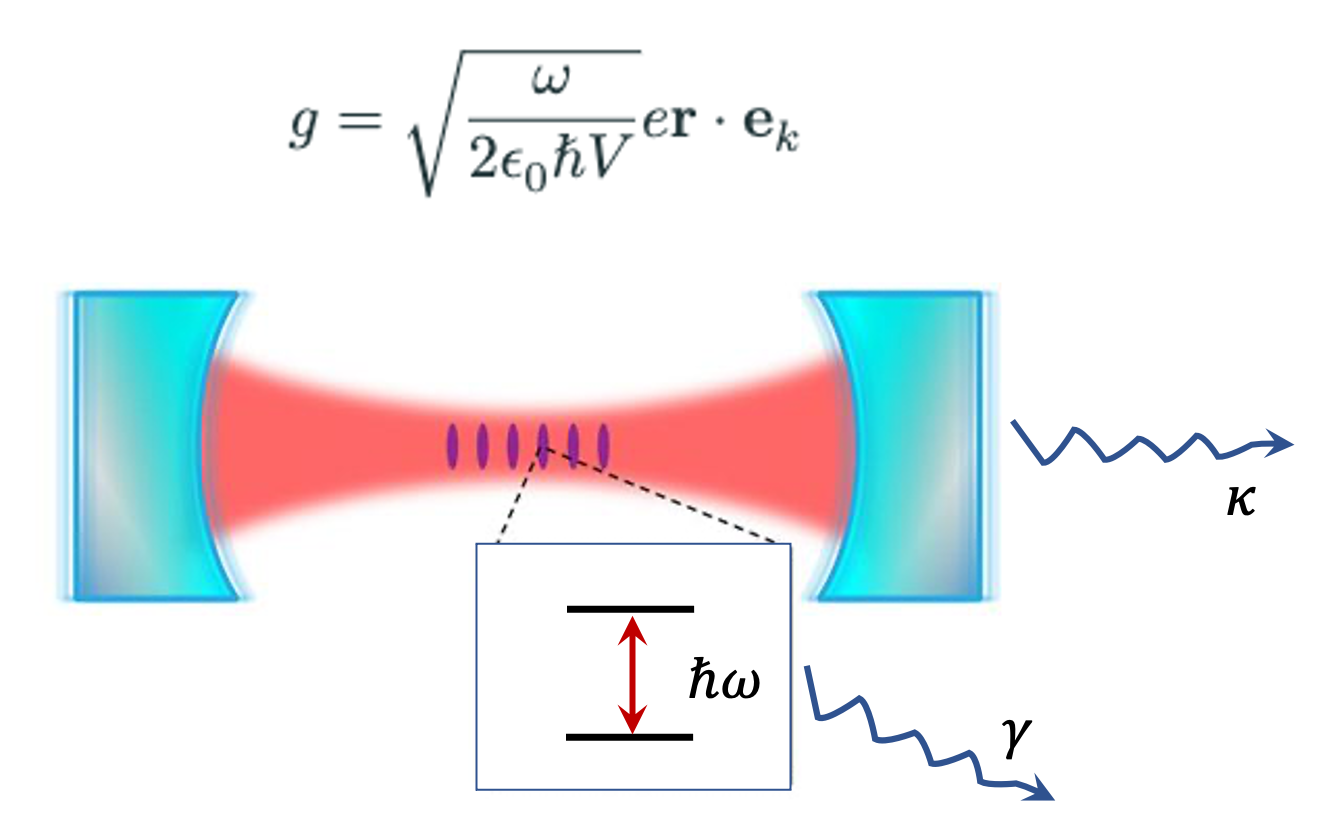
\includegraphics[width=0.6\textwidth]{figs/25.png}
  \end{center}
  想要观察并利用拉比振荡, 必须增强光与原子之间的耦合 $g$. 腔场可最大限度地减少作用体积,增强耦合.
\end{frame}

\section{1. 光学谐振腔}

\begin{frame} 
\frametitle{}   
{\Bullet}光学谐振腔具有选频功能.当不同频率的入射波在腔镜上来回反射时,同频的反射波及入射波之间会相互干涉,腔内稳定传播的都是干涉相长的波.
\begin{columns}[T,onlytextwidth]
    \column{0.59\textwidth}
     考虑fp干涉仪型平面光腔, 透射系数
     \[ T = \frac{1}{1+(4F^2/\pi^2)\sin ^2(\varphi /2)}\]
    式中, 往返相移
    \[ \varphi = \frac{4\pi n L_{cav}}{\lambda}\]
    空腔的精细度
    \[ F = \frac{\pi (R_1 R_2)^{\frac{1}{4}}}{1-\sqrt{R_1 R_2}}\]
    \column{0.4\textwidth}
        \begin{center}
             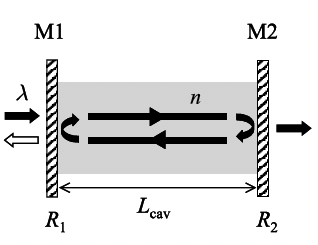
\includegraphics[width=0.9\textwidth]{figs/2022-05-22-23-47-55.png}
        \end{center}
  \end{columns}
\end{frame}

  \begin{frame} 
  \frametitle{}
  \begin{columns}[T,onlytextwidth]
    \column{0.59\textwidth}
       共振透射 ($T=1$) 条件
       \[ \varphi =\frac{4\pi n L_{cav}}{\lambda} = 2 m \pi, \quad m=0, 1, 2, \cdots  \]
       \[L_{cav} = m \frac{\lambda}{2n}\]
       共振模
       \[ \omega_m = m \frac{\pi c }{n L_{cav}}\]
       谱宽
       \[ \Delta \omega = \frac{\pi c }{n F L_{cav}}\]
       品质因数(Q值)
       \[ Q= \frac{\omega}{\Delta \omega }\]
       \column{0.4\textwidth}
       \begin{center}
            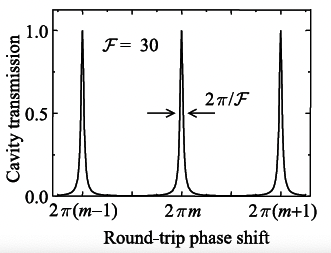
\includegraphics[width=0.9\textwidth]{figs/2022-05-23-00-15-53.png}
       \end{center}
    \end{columns}
  \end{frame}

  \begin{frame} 
  \frametitle{}
    光子衰减率(损失率)
  \[ \boxed{\kappa \equiv  \frac{1}{\tau_{cav}} = \Delta \omega } \]
       光腔共振模的谱宽由光子衰减率决定 \\ {\vspace*{1.3em}}
       原子光谱的谱宽由原子的自发发射率决定.
       \[ \boxed{A_{21} \equiv  \frac{1}{\tau_{a}} = \Delta \omega } \]
  \end{frame}

  \section{2. 原子与腔的相互作用}

\begin{frame} 
\frametitle{}
     
\end{frame}